\documentclass[UTF8,a4paper,11pt,fontset=fandol]{ctexart}
\usepackage{conteststyle}

\begin{document}

\ContestTitle{A3. 轻量 RTL 逻辑综合工具}

{\color{Accent}\bfseries\LARGE 题目描述}\par
\vspace{0.35em}
设计并实现一个可离线构建的 RTL 逻辑综合工具。工具读取 Verilog/SystemVerilog RTL、top module、SDC 和 Nangate45 Liberty，在统一资源限制下生成一个或多个合法门级网表。评测重点依次为网表功能正确性、arrival-area PPA、综合运行时间，以及提交源码的原创贡献。

参赛队必须提交工具源码和统一 Makefile。允许参考或复用 Mockturtle、Yosys、Berkeley ABC 等开源项目，也允许使用大模型辅助开发；所有第三方依赖和开发方式必须如实披露。

\section{核心要求}

\subsection{RTL 前端与 elaboration}

工具应能处理题库使用的 Verilog/SystemVerilog 语法和工程特征，包括：

\begin{itemize}
  \item module 层次、参数化、generate、连续赋值和过程语句；
  \item 组合逻辑、时钟触发逻辑、同步/异步复位和有限状态机；
  \item escaped identifier、宽位向量、signed 运算和生成器产生的 RTL；
  \item 题目 \code{problem.yaml} 给出的 top、clock 和 reset 元数据。
\end{itemize}

\subsection{逻辑优化与技术映射}

工具应完成 RTL 降级、中间表示构建、技术无关优化和 Nangate45 technology mapping。输出网表只能实例化指定 Liberty 中存在的标准单元，不得保留黑盒、未解析的内部 cell 或依赖未提供库的模块。

参赛队可为同一 circuit 输出多种 area/timing 取舍。评测器传入 \code{CONFIG} 和 \code{CIRCUIT} 指定配置文件与题目，再以 \code{POINT} 选择第 1 到第 \(N\) 项，其中 \(1\leq N\leq 7\)。选手工具必须自行解析配置并执行相应优化策略。不同 point 应体现实际综合策略，不得读取题目 ID 后返回预生成网表。

\subsection{源码与可复现构建}

提交必须包含完整可构建源码。评测在指定镜像、无网络环境中从源码执行 \code{make -j1 build}。仅提交二进制、远程 API 包装、缺少许可证的第三方代码或无法离线复现的工程均不符合要求。

\section{交付物}

提交根目录至少包含：

\begin{codebox}[breakable=false,listing options={style=contestcode,basicstyle=\ttfamily\footnotesize}]
Makefile
submission.yaml
config.json
ORIGINALITY_DECLARATION.md
THIRD_PARTY.md
src/
\end{codebox}

\begin{table}[H]
\centering
\begin{tabularx}{\textwidth}{p{0.34\textwidth}Y}
\rowcolor{TableHead}\bfseries 文件 & \bfseries 作用 \\
\code{Makefile} & 评测唯一构建/运行入口，必须实现第 3 节接口。 \\
\code{submission.yaml} & 队伍、工具名称和开发类型。 \\
\code{config.json} & 各 circuit 的 point 参数、优化序列及默认回退配置。 \\
\code{ORIGINALITY\_DECLARATION.md} & 自主模块、开源复用、大模型使用和消融证据。 \\
\code{THIRD\_PARTY.md} & 第三方项目版本、许可证、调用边界和修改情况。 \\
\code{src/} & 工具完整源码及构建所需的本地文件。 \\
\end{tabularx}
\end{table}

模板位于竞赛包 \path{submission_template/}。参赛队可以调整内部目录和命令，但固定 Makefile target、传入变量和输出路径不得修改。

\section{Makefile 测试接口}

评测系统只调用约定的 make target，不依赖提交内部工程结构。

\subsection{必选目标}

\begin{codebox}
build
synth
clean
\end{codebox}

\begin{table}[H]
\centering
\begin{tabularx}{\textwidth}{p{0.20\textwidth}Y}
\rowcolor{TableHead}\bfseries 目标 & \bfseries 作用 \\
\code{build} & 离线编译提交源码，成功后生成可执行入口 \code{bin/synth\_tool}。每份提交构建一次。 \\
\code{synth} & 对一个 circuit 的一个 point 执行综合，并生成规定门级网表。 \\
\code{clean} & 删除提交自己的构建和临时产物，不得删除输入题目或评测目录。 \\
\end{tabularx}
\end{table}

\subsection{参数}

\begin{table}[H]
\centering
\small
\begin{tabularx}{\textwidth}{p{0.16\textwidth}p{0.30\textwidth}Y}
\rowcolor{TableHead}\bfseries 变量 & \bfseries 示例 & \bfseries 含义 \\
\code{RTL} & \code{/case/rtl/design.v} & 输入 RTL 文件，只读。 \\
\code{TOP} & \code{top} & 需要综合且必须保留的顶层模块名。 \\
\code{SDC} & \code{/case/constraints.sdc} & 综合约束，只读。 \\
\code{LIBERTY} & \code{/pdk/Nangate...lib} & 唯一允许的 technology library。 \\
\code{CONFIG} & \code{/submission/config.json} & 提交中的 point 配置文件，只读。 \\
\code{CIRCUIT} & \code{LSV01} & 当前 circuit ID，用于选择配置。 \\
\code{POINT} & \code{1} & 当前优化 point，范围 1 到当前 circuit 的配置值。 \\
\code{OUT\_DIR} & \code{/output} & 当前 point 的独立可写输出目录。 \\
\end{tabularx}
\end{table}

\subsection{每题 Point 数量配置}

提交根目录必须提供标准 JSON 文件 \code{config.json}。顶层 key 是 circuit ID，value 是该 circuit 的 point 配置数组；保留 key \code{\$default} 作为未覆盖题和隐藏题的回退：

\begin{lstlisting}[style=contestcode,frame=single,backgroundcolor=\color{CodeBg},rulecolor=\color{TableBorder}]
{
  "$default": [
    {"name": "balanced", "passes": ["strash", "balance", "rewrite"]}
  ],
  "LSV01": [
    {"abc_sequence": "compress2rs; dch; amap"},
    ["if -K 6 -g -C 8", "dch", "map"]
  ]
}
\end{lstlisting}

每个 value 必须是长度 1--7 的数组，数组长度就是该 circuit 的 point 数量。数组元素可以是任意合法 JSON，包括 object、string、array、number、boolean 或 null；字段名称和执行语义完全由选手定义，可用于表达参数、优化序列、随机种子、映射目标等信息。

评测器只校验顶层映射和数组长度，不解析数组元素，也不会把元素转换成额外命令行参数。工具应读取 \code{CONFIG}，并优先选择键名与 \code{CIRCUIT} 相同的数组；若该键不存在，则选择保留键 \code{\$default} 对应的数组。随后以 \code{POINT-1} 选择并实现当前配置。

评测器对 circuit \(i\) 取得数组长度 \(N_i\) 后，依次调用 \code{POINT=1} 到 \code{POINT=N\_i}。由于选手事先不知道 hidden circuit ID，隐藏题统一使用 \code{\$default} 数组。

\subsection{评测调用流程}

\begin{codebox}
make -j1 build

make -j1 synth \
  RTL=/case/rtl/design.v \
  TOP=top \
  SDC=/case/constraints.sdc \
  LIBERTY=/pdk/NangateOpenCellLibrary_typical.lib \
  CONFIG=/submission/config.json \
  CIRCUIT=LSV01 \
  POINT=1 \
  OUT_DIR=/output
\end{codebox}

成功的 \code{synth} 必须返回 0，并且只需保证以下固定结果存在：

\begin{codebox}
/output/netlist.v
\end{codebox}

\code{netlist.v} 必须非空、可被 Verilog parser 读取，顶层模块名与 \code{TOP} 完全一致。日志可输出到 stdout/stderr；评测系统会统一保存。其他自定义文件不会参与评分。

\begin{noticebox}
评测器对每个 point 使用相同 build snapshot 的独立副本。不得依赖前一个 point 留下的缓存或修改输入文件。失败 point 的运行时间仍计入该 circuit 的总综合时间。
\end{noticebox}

\section{指定环境与资源限制}

指定镜像为 \code{my\_siliconcompiler\_image:latest}，冻结本地 image ID 为：

\begin{codebox}
sha256:cf58004bd15d8d67677812e91ccdebe8da1b17dfab1a0390b96c7f568b74f42a
\end{codebox}

正式比赛通过 Docker Hub、百度网盘 Docker tar 包或预装服务器提供同一镜像。主要参考工具为 Yosys 0.54、OpenSTA 2.7.0、Icarus Verilog 10.3 及 Yosys 随附 Berkeley ABC。

每个综合 point 固定：

\begin{itemize}
  \item 1 个 CPU 核和 1 个综合线程；
  \item 10 GiB 内存；
  \item 网络关闭；
  \item \code{MAKEFLAGS=-j1}，常见 OpenMP/BLAS 线程变量均设为 1。
\end{itemize}

工具主动创建并行综合 worker 属于违规；内存超限或进程异常退出时，该 point 无效。

\section{正确性检查}

正确性是每道题获取分数的前提，而且按 point 单独判定。主办方不会使用选手报告中的“正确”标志，而是执行独立检查：

\begin{enumerate}
  \item 读取 \code{netlist.v}，link 到指定 top，检查没有黑盒和未授权单元；
  \item 使用隐藏 testbench/seed 对原始 RTL 做零延迟仿真，生成 golden trace；
  \item 用同一 testbench/seed 仿真门级网表和 \path{NangateOpenCellLibrary.v} 功能模型；
  \item 对有效采样周期的输出 trace 做逐字节比较。
\end{enumerate}

组合题包含边界与随机向量；时序题先按题目元数据复位，再覆盖正常协议和随机序列。任一规定 seed 不一致即为错误 point。错误 point 不进入 PPA 集合；若某 circuit 没有任何正确 point，该 circuit 得 0 分。

\section{数据集构成}

正式题库共 20 个 circuit：10 个 public 可见题和 10 个 hidden 评测题。20 题等权计分。可见题覆盖组合控制/算术、FSM、AXI 控制、浮点转换、除法、乘法流水、SHA-256 和 RISC-V 小核。

\begin{longtable}{p{0.12\textwidth}p{0.30\textwidth}p{0.22\textwidth}p{0.12\textwidth}r}
\rowcolor{TableHead}\bfseries ID & \bfseries 名称 & \bfseries 类别 & \bfseries 难度 & \bfseries RTL 行数 \\
\endfirsthead
\rowcolor{TableHead}\bfseries ID & \bfseries 名称 & \bfseries 类别 & \bfseries 难度 & \bfseries RTL 行数 \\
\endhead
LSV01 & epfl\_priority & combinational priority & easy & 1102 \\
LSV02 & epfl\_cavlc & combinational control & easy & 766 \\
LSV03 & epfl\_adder & combinational arithmetic & easy & 1206 \\
LSV04 & itc99\_b11 & sequential FSM & medium & 139 \\
LSV05 & sog\_axi\_downsizer & AXI control & easy & 220 \\
LSV06 & sog\_pfpu\_f2i & floating-point conversion & easy & 23 \\
LSV07 & sog\_qdiv & sequential divider & medium & 82 \\
LSV08 & sog\_stage\_mult & multiplier pipeline & medium & 30 \\
LSV09 & sha256\_wishbone & crypto/bus & hard & 1085 \\
LSV10 & vexriscv\_small & CPU core & hard & 3319 \\
\end{longtable}

每题目录包含 \code{rtl/design.v}、\code{constraints.sdc}、\code{problem.yaml} 和简要说明。隐藏题保持相同接口和相近语法/规模分布，不向选手发布 RTL 和参考结果。

\section{官方 Reference Points}

每个 circuit 有 7 个官方 reference points，用于构造 arrival-area Pareto front：5 个 Yosys/ABC point 和 2 个 Design Compiler point。可见题完整结果位于 \path{references/}，Pareto 图位于 \path{figures/public_pareto/}。

\begin{table}[H]
\centering
\small
\begin{tabularx}{\textwidth}{p{0.17\textwidth}Y}
\rowcolor{TableHead}\bfseries Point & \bfseries Reference 策略 \\
\code{yosys\_p1} & \code{compress2rs + dch} 后映射 Nangate45。 \\
\code{yosys\_p2} & \code{if -K 6 -g -C 8 + dch} 后映射 Nangate45。 \\
\code{yosys\_p3} & \code{resyn2rs + dch} 后映射 Nangate45。 \\
\code{yosys\_p4} & 两遍 \code{compress2rs + dch} 后映射 Nangate45。 \\
\code{yosys\_p5} & 两遍 \code{if -K 6 -g -C 8 + dch} 后映射 Nangate45。 \\
\code{dc\_area} & 官方 area-oriented 商业工具 reference，仅用于构造 reference front。 \\
\code{dc\_timing} & 官方 timing-oriented 商业工具 reference，仅用于构造 reference front。 \\
\end{tabularx}
\end{table}

商业 reference 不是参赛环境依赖；提交工具必须能在指定开源镜像中独立构建和运行。

\section{评分机制}

\subsection{统一 PPA 评价}

主办方使用 Nangate45 typical Liberty 和统一 OpenSTA 脚本重新评价所有正确网表。评价 SDC 将 clock period、input/output delay 和 max delay 置 0，同时保留 drive/load 与 reset false path：

\[
  \mathrm{arrival\_ns}=\max(0,-\mathrm{WNS})
\]

Area 为实例化标准单元的 Liberty area 之和。arrival 和 area 都是越小越好。

\subsection{PPA Hypervolume}

对 circuit \(i\)，由官方 7 个成功 points 得到 reference Pareto front \(P_i^{ref}\)。固定 nadir 点为

\[
z_i=\left(1.05\max_{r\in R_i}r_{arrival},\;1.05\max_{r\in R_i}r_{area}\right).
\]

令 \(S_i\) 为选手该题所有正确 points，二维 dominated hypervolume 得分为

\[
Q_i^{PPA}=\min\left(2,\frac{HV(S_i,z_i)}{HV(P_i^{ref},z_i)}\right).
\]

只提交一个 point 时按单元素集合计算；多个互补 point 可覆盖更完整的 area/timing 取舍。Reference front 对应 \(Q_i^{PPA}=1\)，超过 reference 后继续线性加分，达到 2 倍 hypervolume 时封顶；原始 ratio 仍保存用于并列判定。

\begin{figure}[H]
\centering
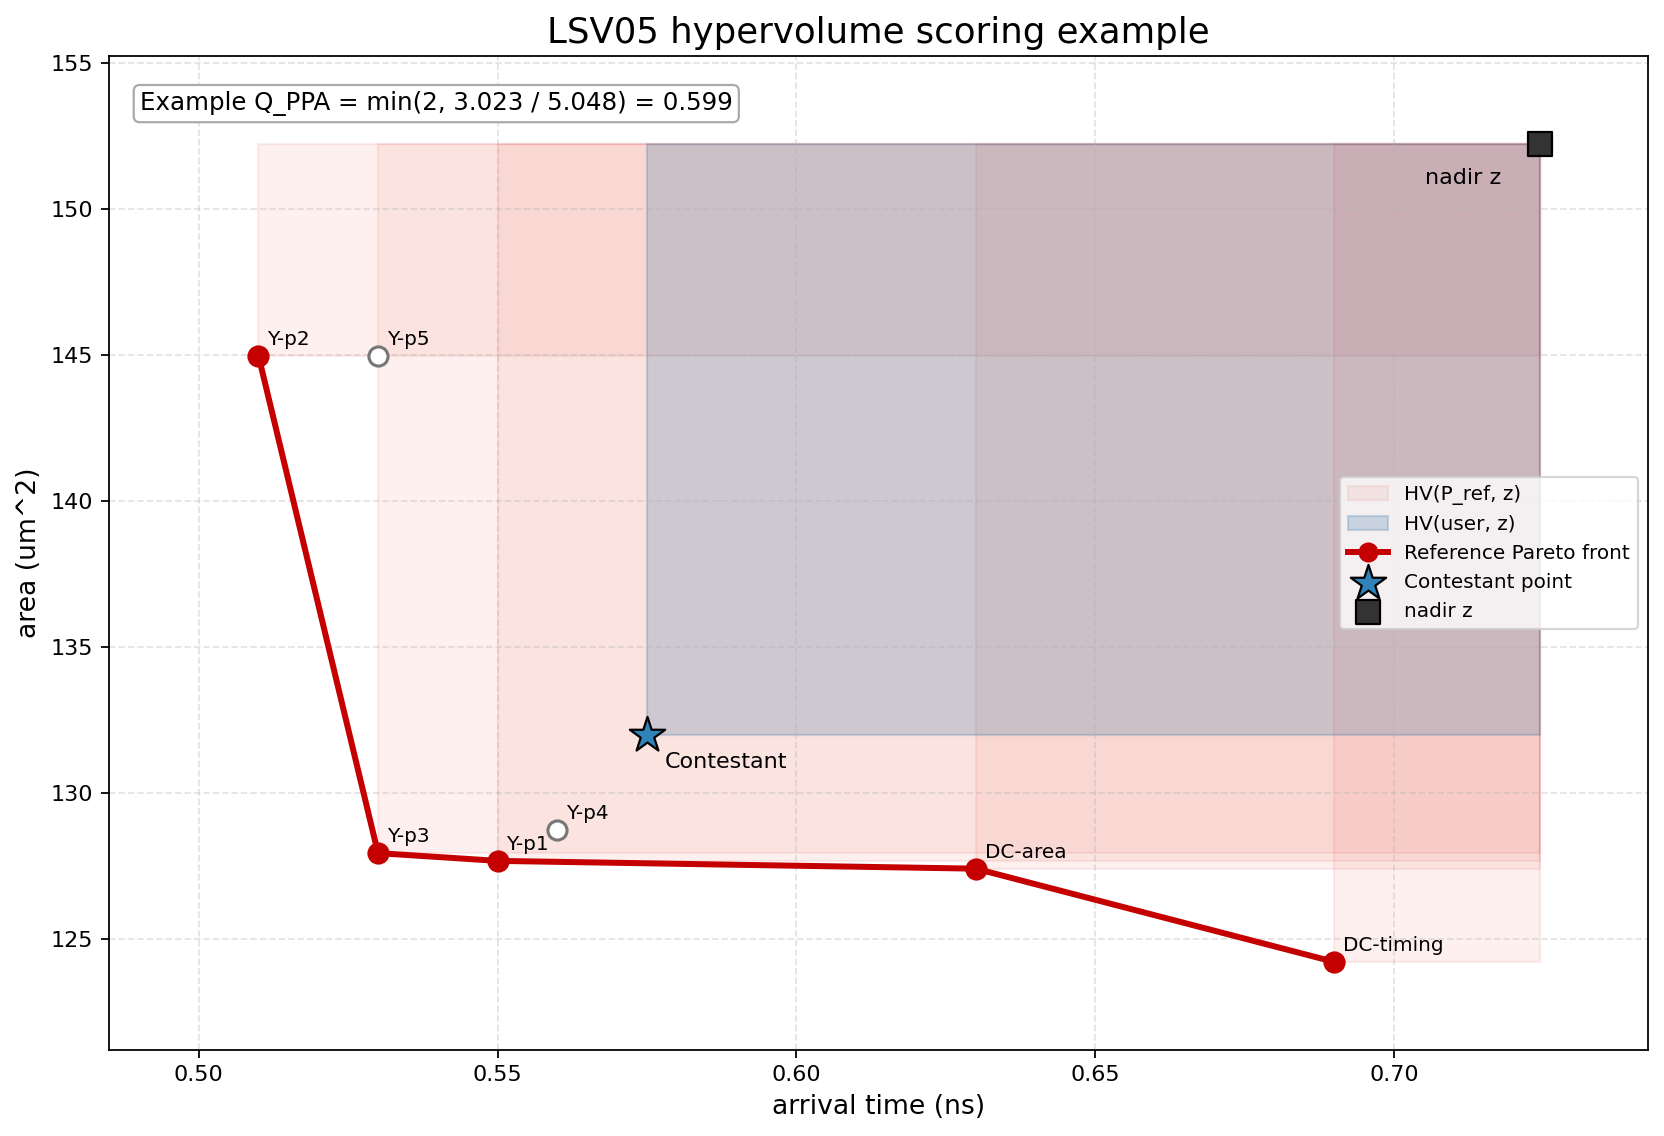
\includegraphics[width=0.78\textwidth]{assets/LSV05_hypervolume_example.png}
\caption{单个选手 point 相对 reference front 的 hypervolume 示意}
\end{figure}

\subsection{Runtime 与单题分}

\(T_i^{ref}\) 为官方 7 个 reference point 的综合 wall time 总和；\(T_i^{user}\) 为选手该题所有尝试 points 的 \code{make synth} wall time 总和，包括失败 point，不包括 build、仿真和 OpenSTA 评价：

\[
Q_i^{time}=\min\left(1,\frac{T_i^{ref}}{T_i^{user}}\right)
\]

\[
Score_i=G_i\left(45Q_i^{PPA}+5Q_i^{time}\right),\qquad
S_{tech}=\frac{1}{20}\sum_{i=1}^{20}Score_i
\]

其中 \(G_i=1\) 表示至少一个 point 通过正确性检查，否则 \(G_i=0\)。单题技术分范围 0--95，20 题均值 \(S_{tech}\) 也为 0--95；其中 PPA 最多 90 分，runtime 最多 5 分。

当提交 hypervolume 等于 reference 且 runtime 不慢于 reference 时，该题得到 50 分；达到 2 倍 reference hypervolume 且 runtime 满分时，该题得到 95 分。

\subsection{原创性附加分}

参赛队在 \code{submission.yaml} 二选一声明：

\begin{itemize}
  \item \code{open\_source\_based}：基于/调用开源 EDA 工具开发；
  \item \code{from\_scratch}：综合核心链路由队伍自主实现。
\end{itemize}

两类技术评分完全相同。原创性由源码自主性、算法贡献、核心完整度、消融证据、可复现与答辩五项审核，每项 0 到 1 分：

\[
S_{final}=S_{tech}+S_{originality}\leq100,\qquad 0\leq S_{originality}\leq5.
\]

因此最终总分固定为 100 分：PPA 90、runtime 5、原创性 5。

开源工具自身能力不计作本队原创贡献，但在其上实现的新 pass、代价模型、搜索方法和映射算法可据证据评分。大模型辅助开发不自动扣分，须披露并能解释、复现和维护相关代码。

\section{开源工具参考与行为边界}

可参考的项目包括但不限于：

\begin{itemize}
  \item Mockturtle：逻辑网络表示、重写、重代数和映射研究；
  \item Yosys：Verilog 前端、RTL lowering、基础综合和 Liberty 接口；
  \item Berkeley ABC：AIG 优化、cut-based mapping 和标准综合序列。
\end{itemize}

使用这些项目必须遵守许可证，在 \code{THIRD\_PARTY.md} 固定版本/commit，并在原创声明中划清上游代码与自主代码。禁止未披露复制其他队伍代码、调用评测服务器外部服务、读取隐藏题标识做特化或提交预计算 netlist。

\begin{noticebox}
{\small\textbf{提交前检查：}指定镜像可离线执行 \code{make -j1 build}，且 \code{bin/synth\_tool} 可执行；10 道可见题的全部声明 points 均生成规定 \code{netlist.v}；top 与标准单元合法；每 point 满足 1 核、1 线程和 10 GiB；point 数量、开发类型、原创内容、第三方许可证、大模型使用和消融证据均已准确披露。}
\end{noticebox}

\end{document}
